\chapter{Experiments} \label{sec:experiments}
In this section, we investigate the effectiveness of the proposed framework $MGTCOM$ (in \cref{sec:approach}) by evaluating its performance on auxiliary tasks related to multimodal networks.
We start by describing our experimental setup, whereafter we compare the performance of our model against baseline methods.

\section{Evaluation metrics}
There are no measures that can assess the quality of communities in multimodal networks.
Therefore, we evaluate our model component-wise by defining related auxiliary tasks. 
On a high level, these tasks evaluate the efficiency of topological and temporal node embeddings and found communities. 
The found communities shall capture important patterns in the data which are useful for further analysis.
%
In order to measure predictive performance over distinct aspects of our data, we first define the following labels for calculating performance metrics, then describe the auxiliary tasks.

\begin{itemize}[leftmargin=*]
    \item \textbf{Ground truth labels $L_y$}. 
    Various datasets include manually selected ground truth labels which capture valuable higher-order relations within data. By measuring prediction performance on this label we gauge the quality of found communities.
    \item \textbf{Node timestamps $L_\mathcal{T}$}. 
    We split the nodes evenly into snapshot labels given the timestamp of their first occurrences. This allows measuring the quality of node embeddings on temporal prediction.  
    \item \textbf{Link-based communities $L_G$}. 
    While other measures such as modularity and link prediction are well-suited for measuring the quality of node embeddings in capturing the structure of a given network, they either require community assignment or measure low-proximity similarity.
    In order to overcome this, we first identify community labels using the Louvain method~\cite{blondelFastUnfoldingCommunities2008}. Then we use those labels to assess the quality of individual node embeddings for community detection. 
    As the Louvain method greedily approximates optimal communities, we don't use this label for formal comparison.
\end{itemize}


\subsection{Classification (CF)}
In the classification experiment, we  evaluate predictive performance given task-related labels.
To elaborate, given a set of node embeddings and their respective ground truth labels, we train a logistic regression model to predict node labels. 
For the predicted node labels, we calculate the average accuracy classification measure.

\subsection{Link prediction (LP)}
In this set of experiments, we evaluate link prediction performance. 
Given a set of positive and negative node pairs, binary classification is used to predict whether an edge exists within the graph.
We use a held-out positive and randomly sampled negative sets of edges to train a logistic regression model.
The inner-product similarity between a pair of node embeddings is used as input for the model.
By repeating this process three times, the average accuracy is calculated.

\subsection{Cluster quality}
Given node embeddings and their respective labeling,  we calculate the silhouette coefficient and Davies-Bouldin index which are helpful to estimate how coherent a clustering is.
In this case, a coherent clustering indicates how well represented the correlated patterns are within the embeddings.

\begin{secDefinition}[\textbf{Davies-Bouldin Index}]\label{def:dbi}
Davies-Bouldin Index (DBI) is the ratio of the sum of the average distance to the distance between the centers of mass of the two clusters. 
In other words, it is defined as a ratio of within-cluster, to the between cluster separation. 
This measure is defined as an average over all the found clusters and is therefore also a good measure to decide how many clusters should be used (See \cref{eq:dbi_r,eq:dbi}).
The $s_i$ refers to the average distance between each point in cluster $i$ to its cluster center $\mu_i$, and $dist(\boldsymbol{\mu}_i, \boldsymbol{\mu}_j)$ refers to the distance between cluster centers $\mu_i$ and $\mu_j$.
Since we use inner-product for node similarity, we define inner-product distance as \cref{eq:dotpdist}.

\begin{align}
    dist(\textbf{Z}_i, \textbf{Z}_j) &= -\sum_{m=0}^d Z_{im}Z_{jm} \label{eq:dotpdist}\\
    R_{i j} &=\frac{s_{i}+s_{j}}{dist(\boldsymbol{\mu}_i, \boldsymbol{\mu}_j)} \label{eq:dbi_r} \\
    DBI &=\frac{1}{k} \sum_{i=1}^{K} \max _{i \neq j} R_{i j} \label{eq:dbi} \\
\end{align}
\end{secDefinition}

\subsection{Link-based Community quality}
In this experiment, we measure link-based community quality.
Girvan and Newman \cite{girvanCommunityStructureSocial2002} defined community structure as a group of nodes where inter-community connectivity is higher than intra-connectivity. 
Following this definition, they introduce a modularity measure to evaluate the quality of found communities in a given network. We make use of this measure in our empirical evaluation. Note that we use modularity (\cref{def:modularity}) to measure the quality of topological communities. 

\begin{secDefinition}[\textbf{Modularity}]\label{def:modularity}
Modularity directly measures the density of links inside a graph and is therefore computed on communities (sets of nodes) individually by weighing edges using community similarity (or exact matching). 
Calculation of modularity is done by aggregating per community $r$ for each pair of nodes $v$ and $w$ the difference between the expected connectivity $\frac{k_{v} k_{w}}{2 m}$ (expected amount of edges between the nodes) and the actual connectivity $A_{vw}$ (existence of an edge) given their degrees ($k_v$ and $k_w$). 
The final result represents the connectivity difference between the current and a random graph, as expected connectivity is determined by random rewirings. 
Because intracommunity pairs are weighted less than intercommunity pairs, the score can vary. 
See \cref{eq:modularity}, where $S_{vr}$ denotes membership of node $v$ to community $r$ (\cref{eq:mod_membership}), and $m$ represents the total edge count.

\begin{align}
    Q &=\frac{1}{2 m}\sum_{v w}\sum_{r}\left[\overbrace{A_{v w}}^{\text{Connectivity}}-\underbrace{\frac{k_{v} k_{w}}{2 m}}_{\text{Expected Connectivity}}\right] \overbrace{S_{v r} S_{w r}}^{\text{Community Similarity}} \label{eq:modularity} \\
    S_{vr} &= \begin{cases}
        1 & \mathbf{z}_v = r \\
        0 & \text{otherwise}
    \end{cases} \label{eq:mod_membership}
\end{align}
\end{secDefinition}

\subsection{Ground-truth community quality (COM)}
Similarly, to measure the quality of detected communities for specific tasks, we measure the Normalized Mutual Information Score (NMI) score given a task-based label (\cref{def:nmi}).

\begin{secDefinition}[\textbf{Normalized Mutual Information Score (NMI)}]\label{def:nmi}
Normalized Mutual Information is a popular measure used to evaluate network partitioning. 
It is a variant of a common measure in information theory called Mutual Information defined by $I(X; Y) = H(X) - H(X| Y)$ and represents a reduction in entropy $H(X)$ of variable $X$ by observing the random variable $Y$ or vice versa.
In the context of ground-truth community evaluation setting this measure is used to quantify the overlap between two sets of partitions.
The Mutual Information score for two sets of partitions $X$ and $Y$ is computed using \cref{eq:mi}, where $|X|$ is the size of set $X$, $X_i$ refers to $i$'th partition of set $X$, and $N$ is the total number of data points.
Finally, the NMI score is computed by normalizing the MI score using the arithmetic mean of entropy of respective partitions \cref{eq:nmi}.

\begin{align}
    MI(X; Y) &= \sum_{i=1}^{|X|} \sum_{j=1}^{|Y|} \frac{\left|X_{i} \cap Y_{j}\right|}{N} \log \frac{N\left|X_{i} \cap Y_{j}\right|}{\left|X_{i}\right|\left|Y_{j}\right|} \label{eq:mi} \\
    NMI(X; Y) &= \frac{MI(X; Y)}{(H(X) + H(Y)) / 2} \label{eq:nmi}
\end{align}

\end{secDefinition}

\section{Experimental setup} \label{sec:exp_setup}
As shown in \cref{tab:comparison_related_work} of \cref{sec:related_work} there are no directly comparable methods to ours in terms of features.
For a fair and coherent comparison, we define three variants of the MGTCOM model for evaluation.
In addition to the complete end-to-end model $MGTCOM$, we split our framework into a temporal model $MGTCOM^{\mathcal{T}}$ and topological model $MGTCOM^{\mathcal{E}}$, by removing $\mathcal{L}_{\mathcal{T}}$ and $\mathcal{L}_{\mathcal{E}}$ from the objective respectively.

For evaluation, we split the network edges into disjoint training (80\%), validation (10\%), and testing (10\%) sets.  
During link prediction, we exclusively use links in the respective set as positive pairs.
Negative pairs are sampled given the full set of edges.
Similarly, the clustering is computed on the training embeddings while cluster-based metrics are calculated using test and validation sets.
During the calculation of predictive metrics such as link prediction and classification, we run logistic regression three times and use the average to get an accurate measurement.

\subsection{Hyperparameters}
The hyperparameters for $MGTCOM$ model can be attributed to either network architecture, topological random walk, temporal random walk or clustering.
In \cref{sec:abl:hyperparam} we explore the sensitivity of our model to these hyperparameters.
In \cref{sec:supplemental} we display a complete overview of all the hyperparameter values used for evaluation.
The most important hyperparameters are specified below.

For primary embedding, we use two HGT layers with neighborhood sampling sizes of 8 and 4.
All the hidden dimensions are equal to the representation dimension, which is 64 ($d=64$).
For temporal and topological context sampling we use walk length $l=10$ with 10 walks per node.
Node2Vec is configured to use $q=0.5$ to favor neighborhood exploration. 
The temporal sampling window $\omega$ for ballroom walk is determined for each dataset by splitting $\mathcal{T}$ into 20 even partitions.
For the clustering module we define prior parameters as $\nu = d + 1, \kappa = 1, \alpha = 10$ and $\Sigma_{scale} = 0.05$.
We set trade-off parameters as $\beta^{\mathcal{E}} = 1, \beta^{\mathcal{T}} = 1, \beta^{C} = 0.01$. 
For max-margin loss we set $\Delta$ to $0.1$.

\subsection{Baselines} 
We use various graph embeddings and community detection algorithms as baselines, covering state-of-art developments in related fields.
For the baselines, we use the hyperparameters reported in their respective papers. 
To keep the results comparable, we use representation dimension $d=64$ throughout.

\begin{itemize}[leftmargin=*]
    \item \textbf{ComE \cite{cavallariLearningCommunityEmbedding2017}} uses Gaussian mixture model to learn homogeneous graph embeddings and cluster parameters jointly while utilizing random walk based context sampling.
    \item \textbf{GEMSEC \cite{rozemberczkiGEMSECGraphEmbedding2019}} uses random walks to learn community structure and embeddings simultaneously on homogeneous graphs.
    \item \textbf{CP-GNN \cite{luoDetectingCommunitiesHeterogeneous2021} } learns node embeddings from a heterogeneous graph by utilizing transformers and k-hop context sampling.
    \item \textbf{CTDNE \cite{nguyenContinuousTimeDynamicNetwork2018} } utilizes time-based biased random walks to learn spatio-temporal node representations from dynamic networks. 
    \item \textbf{GraphSAGE \cite{hamiltonInductiveRepresentationLearning2017} } uses k-hop neighborhood sampling to learn node embeddings from homogeneous graphs. Its unsupervised variant combines contrastive link sampling with hinge loss.  
    \item \textbf{Node2Vec \cite{groverNode2vecScalableFeature2016}} adopts biased random walk and Skip-Gram to learn node embeddings from homogeneous graphs.
\end{itemize}

\subsection{Datasets} 
\begin{table}[ht!]
\centering
\caption{
Dataset statistics. 
\textit{Temporal} indicates if a dataset is temporal and \textit{labelled} refers to the availability of ground truth labels.  
}
\label{tab:datasets}
\small
% \resizebox{\columnwidth}{!}{
\begin{tabular}{@{}ccccccc@{}}
    \toprule
    Dataset                 & Node type     & \# Nodes  & Edge type             & \# Edges  & Temporal                      & Labelled \\
    \midrule
    \multirow{3}{*}{DBLP}   & Author (A)    & 5,162     & A - Authored - P      & 11,022    & \multirow{3}{*}{$\bullet$}    & \multirow{3}{*}{$\bullet$}\\
                            & Paper (P)     & 5,511     & P - Published In - V  & 5,511     &                               &                           \\
                            & Venue (V)     & 14        &                       &           &                               &                           \\ \midrule
    \multirow{3}{*}{IMDB}   & Person (P)    & 8,491     & P - Directed - M      & 4,939     & \multirow{3}{*}{$\bullet$}    & \multirow{3}{*}{}         \\ 
                            & Movie (M)     & 5,043     & P - Acted In - M      & 15,086    &                               &                           \\
                            & Genre (G)     & 26        & M - Tagged   - G      & 14,504    &                               &                           \\ \midrule
    \multirow{7}{*}{SDS}    & User (U)      & 34,919    & U - Tweeted  - T      & 56,173    & \multirow{7}{*}{$\bullet$}    & \multirow{7}{*}{}         \\ 
                            & Hashtag (H)   & 2,341     & T - Reply To - U      & 21,769    &                               &                           \\
                            & Tweet (T)     & 56,173    & T - Reply To - T      & 4,296     &                               &                           \\
                            &               &           & T - Quote    - T      & 882       &                               &                           \\
                            &               &           & T - Mention  - U      & 70,367    &                               &                           \\
                            &               &           & T - Mention  - H      & 12,313    &                               &                           \\
                            &               &           & U - Follows  - U      & 5,649,098 &                               &                           \\ \midrule
    \multirow{1}{*}{ICEWS}  & Entity (E)    & 10,463    & 123 different types   & 915,028   & \multirow{1}{*}{$\bullet$}    & \multirow{1}{*}{}         \\ \midrule
    \multirow{1}{*}{Cora}   & Paper (P)     & 2,708     & P - Cites - P         & 10556     & \multirow{1}{*}{}             & \multirow{1}{*}{$\bullet$}\\ 
    \bottomrule
\end{tabular}
% }
\end{table}

We use four widely used real-world (temporal) datasets for evaluation.
These graphs are of different types and contain information on different modalities.
We applied additional preprocessing on the IMDB, DBLP-HCN, and ICEWS datasets to include the multimodal features present in the datasets but often not included in the graph due to sparsity of temporal or content-based features. 
See \cref{tab:datasets} for a detailed comparison of node features.

\begin{itemize}[leftmargin=*]
    \item \textbf{DBLP} \cite{yangDefiningEvaluatingNetwork2012} is a citation network consisting of Authors, Papers and Venues. Aside from being heterogeneous, the dataset also contains timestamps representing paper publication dates and abstracts. There are thirteen ground-truth communities representing publication venues. The  network contains 10687 nodes and 33066 edges. This dataset includes ground truth labels.
    \item \textbf{ICEWS} \cite{garcia-duranLearningSequenceEncoders2018}
    is a temporal knowledge graph in which nodes represent entities and timestamped edges the relationship between them. We model this data as a highly heterogeneous network consisting of different types of nodes (10463 in total) connected by 915028 timestamped edges. Edges are labeled with relations. 
    \item \textbf{IMDB5000} \cite{IMDB5000Movie} network consists of Actor, Director, Movie, and Genre nodes where each Movie node type has a timestamp denoting the release date. Additionally, each actor node has a set of attributes characterizing information unique to the actor such as age and popularity, while movies have box-office data and keywords encoded as feature vectors. This network has 13560 nodes and 69058 edges. 
    \item \textbf{SocialDistancingStudents (SDS)} \cite{wangPublicSentimentGovernmental2020} represents a small part of the Twitter network around a set of hashtags related to the COVID pandemic. This heterogeneous network models connections between Users, Tweets, and Hashtags where parallel edges are possible due to relations such as tweeted, retweeted, quoted, etc. The tweet nodes contain publication date timestamps and content encoded as feature vectors. 93433 nodes and 7420366 edges are included. 
   \item \textbf{Cora} \cite{yangRevisitingSemisupervisedLearning2016} is a homogeneous citation network. Nodes represent published papers and contain feature vectors representing specific term occurrences in the abstract. Each node is associated with one of the seven ground-truth labels. 
\end{itemize}

%=====================================================================================
\section{Performance comparison}
\begin{table*}[t!]
\centering
\caption{
    Comparison of performance of baselines on multimodal graph learning tasks. 
    ("-" means no data available, for example for temporal methods on static datasets such as Cora).
    The calculated metrics are the link prediction accuracy ($LP_{ACC}$), predictive accuracy on ground truth communities $CF_{ACC}$ $L_y$, timestamp predictive accuracy $CF_{ACC}$ $L_\mathcal{T}$, NMI score of detected communities ($COM_{NMI}$) given predefined communities ($L_y$, $L_\mathcal{T}$, $L_G$), Davies-Bouldin Index (DBI) and Modularity.
}
\label{tab:results_perf}
% \resizebox{0.86\textwidth}{!}{
\resizebox{\textwidth}{!}{
\begin{tabular}{ccccccccccc}
\toprule
Dataset    &                        & GraphSAGE & Node2Vec      &   ComE        & GEMSEC    &  CTDNE    &  CP-GNN   & $MGTCOM$  & $MGTCOM^{\mathcal{T}}$ & $MGTCOM^{\mathcal{E}}$ \\
\midrule
\multirow{8}{*}{DBLP}
    & $LP_{ACC}$                    & 0.624     & 0.710         & 0.735         & 0.544     & 0.701     & 0.522     & 0.743         & 0.634  & \textbf{0.794} \\
    & $CF_{ACC}$ $L_y$              & 0.315     & 0.832         & 0.842         & 0.831     & 0.809     & 0.506     &\textbf{0.896} & 0.330  & 0.884 \\
    & $CF_{ACC}$ $L_\mathcal{T}$    & 0.309     & 0.308         & 0.328         & 0.324     & 0.488     & 0.313     &\textbf{0.758} & 0.508  & 0.320 \\
    & $COM_{NMI}$ $L_y$             & 0.051     &\textbf{0.549} & 0.463         & 0.385     & 0.537     & 0.209     & 0.465         & 0.059  & 0.492 \\
    & $COM_{NMI}$ $L_\mathcal{T}$   & 0.006     & 0.033         & 0.025         & 0.022     & 0.059     & 0.022     &\textbf{0.209} & 0.168  & 0.026 \\
    & $COM_{NMI}$ $L_G$             & 0.040     & 0.425         &\textbf{0.470} & 0.314     & 0.401     & 0.107     & 0.336         & 0.039  & 0.371 \\
    & DBI                           & 0.472     & 2.305         & 2.205         & 4.056     & 1.206     & 4.780     & 2.039         & 4.205  & \textbf{5.188} \\
    & Modularity                    & 0.028     &\textbf{0.662} & 0.636         & 0.492     & 0.642     &-0.035     & 0.427         & 0.137  & 0.514 \\ \midrule
\multirow{6}{*}{ICEWS}
    & $LP_{ACC}$                    & 0.525     & 0.936         & 0.880         & 0.768     & 0.921     & 0.709     & 0.903         & 0.896  & \textbf{0.945}   \\
    & $CF_{ACC}$ $L_\mathcal{T}$    & 0.294     & 0.301         & 0.264         & 0.310     & 0.285     & 0.273     & 0.316         &\textbf{0.318} & 0.313     \\
    & $COM_{NMI}$ $L_\mathcal{T}$   & 0.018     & 0.040         & 0.015         & 0.022     & 0.022     & 0.013     &\textbf{0.057} & 0.002  & 0.011            \\
    & $COM_{NMI}$ $L_G$             & 0.227     & 0.354         & \textbf{0.548}& 0.309     & 0.347     & 0.204     & 0.119         & 0.001  & 0.447            \\
    & DBI                           & 1.027     & 1.697         & 2.559         & 3.867     & 1.533     &\textbf{4.737}& 3.883      & 3.598  & 3.182            \\
    & Modularity                    & 0.218     & 0.215         & \textbf{0.483}& 0.311     & 0.239     & 0.199     & 0.007         & 0.001  & 0.390            \\ \midrule
\multirow{6}{*}{IMDB}
    & $LP_{ACC}$                    & 0.714     & 0.757         & 0.666         & 0.637     & 0.728     & 0.598     & 0.721         & 0.724  & \textbf{0.773} \\
    & $CF_{ACC}$ $L_\mathcal{T}$    & 0.346     & 0.373         & 0.394         & 0.380     & 0.488     & 0.316     &\textbf{0.659} & 0.556  & 0.377 \\
    & $COM_{NMI}$ $L_\mathcal{T}$   & 0.022     & 0.025         & 0.031         & 0.013     & 0.065     & 0.004     &\textbf{0.239} & 0.231  & 0.026 \\
    & $COM_{NMI}$ $L_G$             & 0.039     & 0.181         &\textbf{0.197} & 0.094     & 0.160     & 0.033     & 0.107         & 0.031  & 0.158 \\
    & DBI                           & 0.301     & 1.803         & 3.840         &\textbf{4.951}& 1.749  & 4.806     & 2.257         & 1.285  & 4.013 \\
    & Modularity                    &-0.172     & 0.190         &\textbf{0.395} & 0.073     & 0.196     & 0.053     & 0.119         & 0.114  & 0.286 \\\midrule
\multirow{6}{*}{SDS}
    & $LP_{ACC}$                    & 0.922     & 0.953         & 0.758         & 0.878     & 0.955     &     -     & 0.934         & 0.616  & \textbf{0.956} \\
    & $CF_{ACC}$ $L_\mathcal{T}$    & 0.521     & 0.445         & 0.386         & 0.384     & 0.447     &     -     & 0.523         & \textbf{0.887}& 0.492 \\
    & $COM_{NMI}$ $L_\mathcal{T}$   & 0.250     & 0.149         & 0.117         & 0.015     & 0.161     &     -     & 0.204         & \textbf{0.536}  & 0.044 \\
    & $COM_{NMI}$ $L_G$             & 0.186     & 0.277         & 0.346         & 0.117     & 0.233     &     -     & 0.120         & 0.043  & \textbf{0.389} \\
    & DBI                           & 1.108     & 2.355         & \textbf{3.986}& 3.410     & 2.890     &     -     & 2.474         & 1.519  & 2.559 \\
    & Modularity                    & 0.088     & 0.163         & 0.301         & 0.037     & 0.016     &     -     & 0.015         & 0.005  & \textbf{0.374} \\\midrule
\multirow{6}{*}{Cora} 
    & $LP_{ACC}$                    & 0.505     & 0.939         &\textbf{0.962} &0.923      & -         & 0.829     & -             & -     & 0.958 \\
    & $CF_{ACC}$ $L_y$              & 0.659     & 0.798         &\textbf{0.864} &0.845      & -         & 0.780     & -             & -     & 0.854 \\
    & $COM_{NMI}$ $L_y$             & 0.376     & 0.345         & 0.434         & 0.437     & -         & 0.370     & -             & -     &\textbf{0.439} \\
    & $COM_{NMI}$ $L_G$             & 0.507     & 0.543         & 0.635         & 0.632     & -         & 0.501     & -             & -     &\textbf{0.643} \\
    & DBI                           & 1.526     & 1.250         & 2.021         & 1.500     & -         & 2.634     & -             & -     &\textbf{2.647} \\
    & Modularity                    & 0.636     & 0.691         &\textbf{0.785} &  0.780    & -         & 0.677     & -             & -     &0.754 \\
\bottomrule
\end{tabular}
}
\end{table*}




In this experiment, we evaluate the performance of learned node embeddings and detected clusters.
In particular, we evaluate the predictive quality of embeddings using classification and link prediction, i.e., link prediction accuracy ($LP_{ACC}$), temporal $L_\mathcal{T}$ and ground truth $L_y$  label classification accuracy $CF_{ACC}$.
We evaluate the quality of detected clusters by calculating their NMI score based on predefined ground-truth communities $L_y$, $L_\mathcal{T}$, $L_G$.
This tells us whether detected clusters approximate user-defined communities $L_y$, temporal partitioning $L_\mathcal{T}$ or the topology $L_G$.
Additionally, we calculate cluster and community quality scores for the learned community assignments, specifically Davies Bouldin score and modularity.

The embeddings obtained from non-community detection methods were clustered using k-means clustering with $K=20$. Similarly, we use $K=20$ for community detection methods (ComE, GEMSEC, CP-GNN) that assume a predefined cluster count.
%
The results are reported in \cref{tab:results_perf}. 
It can be seen that while MGTCOM is competitive on task-specific measures such as link prediction and timestamp prediction, the community detection methods still have an edge on link-based modularity measures. 
A possible explanation for this would be the fact that the DPMM process is more prone to getting stuck in local minima as the clusters split and merge.
Another possibility is that node features do not contain enough information to model very specific network features such as modularity.
In \cref{sec:abl:aux_emb} we further explore this issue by varying the auxiliary embedding ratio.

While CTDNE performs comparatively well in capturing the temporal aspect of the network, we see that it still yields inferior results on datasets where temporal features are weakly correlated with topology.

It is interesting to note that algorithms that rely on pairwise loss measures such as GraphSAGE and CP-GNN perform relatively well on classification-based measures while performing very poorly on cluster quality measures such as DBI and modularity.
A possible explanation for such observation is that the combination of neighborhood sampling and pairwise loss reinforces structural similarity despite having a large receptive field.
Our method successfully overcomes this issue by modifying Hinge loss to work in a context path setting (See \cref{sec:obj_fn}).

We also observe that the MGTCOM model performs well on both topology and temporal prediction tasks in comparison to its task-specific counterparts. 

%=====================================================================================
\section{Qualitative results}
\begin{figure*}[t!]
\centering
% 45 for single column
\subfigure[$MGTCOM$ + $L_y$]{
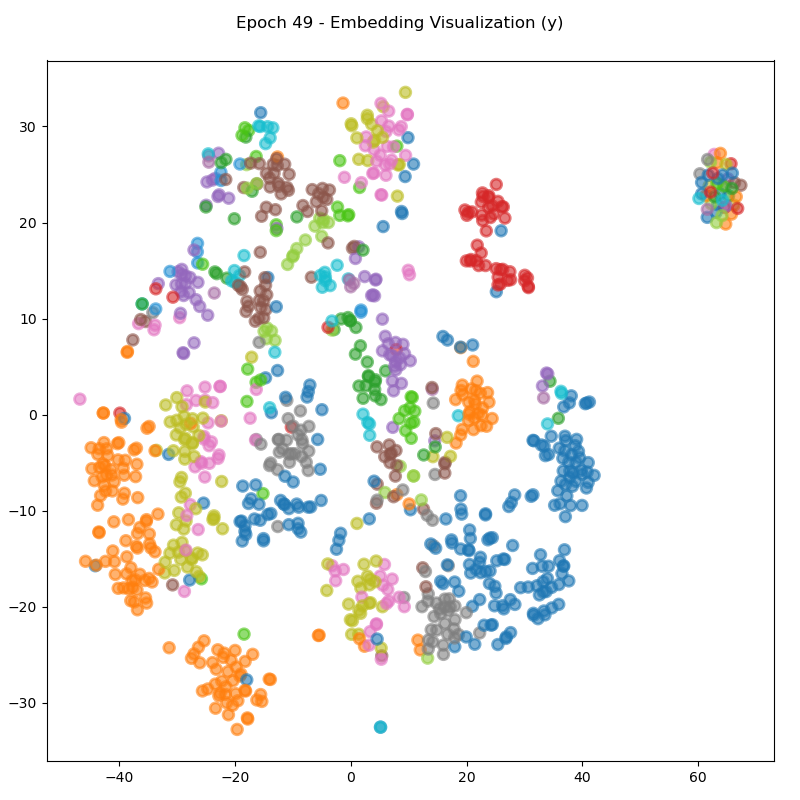
\includegraphics[width=0.23\columnwidth]{resources/visualization/combi_y.png}
}
\subfigure[$MGTCOM$ + $L_{\mathcal{T}}$]{
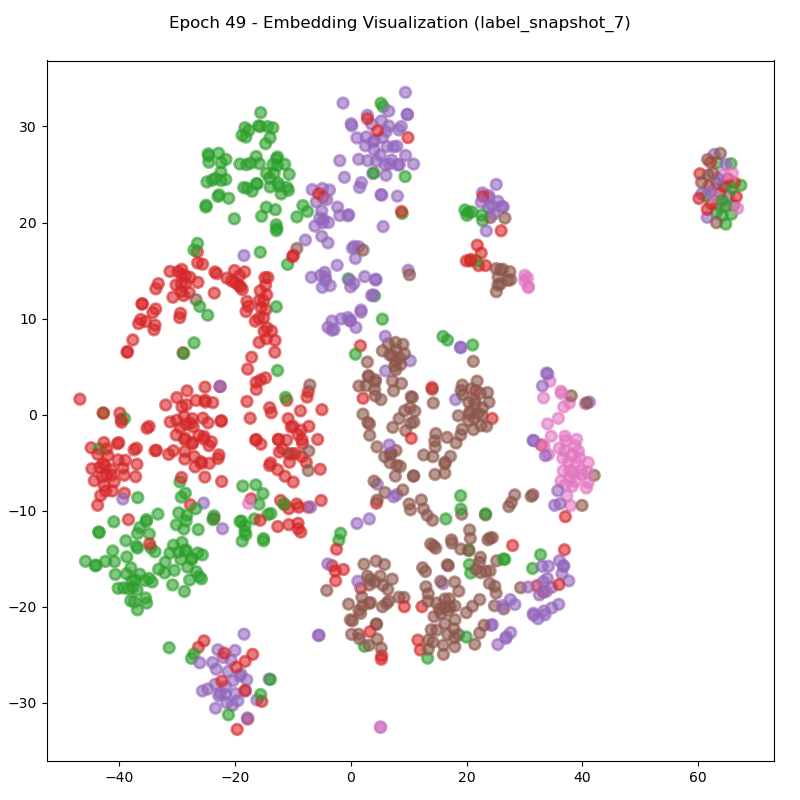
\includegraphics[width=0.23\columnwidth]{resources/visualization/combi_t.png}
}
\subfigure[$ComE$ + $L_y$]{
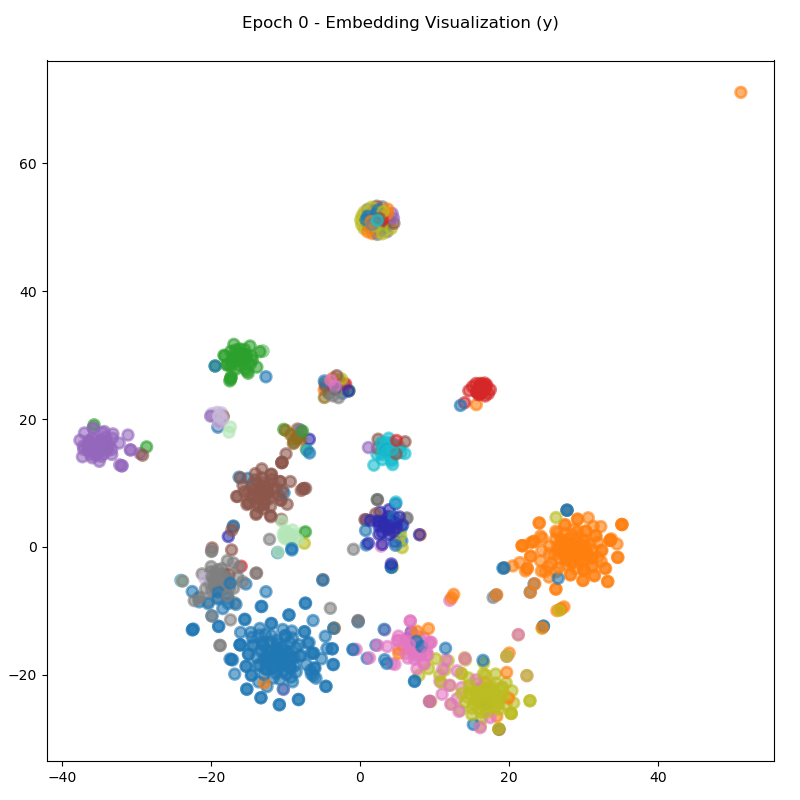
\includegraphics[width=0.23\columnwidth]{resources/visualization/come_y.png}
}
\subfigure[$ComE$ + $L_{\mathcal{T}}$]{
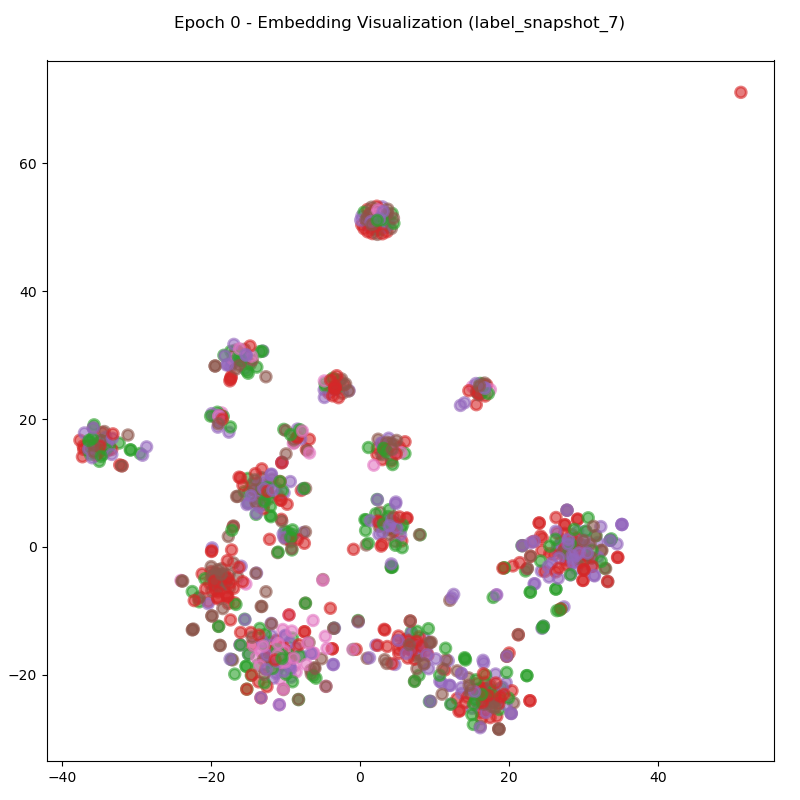
\includegraphics[width=0.23\columnwidth]{resources/visualization/come_t.png}
}\\

\centering
\subfigure[$Node2Vec$ + $L_y$]{
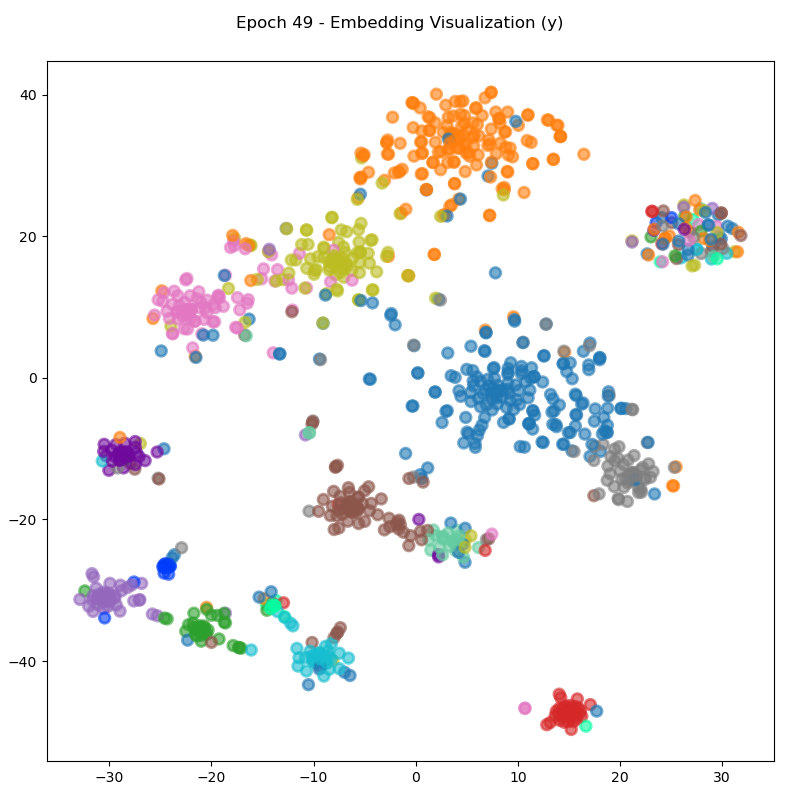
\includegraphics[width=0.23\columnwidth]{resources/visualization/n2v_y.png}
}
\subfigure[$Node2Vec$ + $L_{\mathcal{T}}$]{
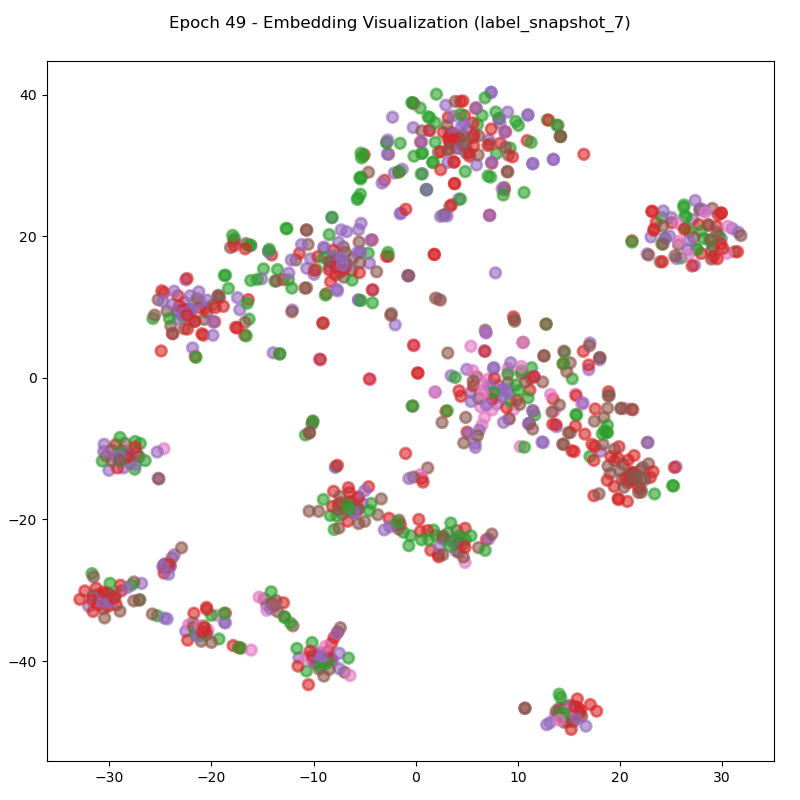
\includegraphics[width=0.23\columnwidth]{resources/visualization/n2v_t.png}
}
\subfigure[$CTDNE$ + $L_y$]{
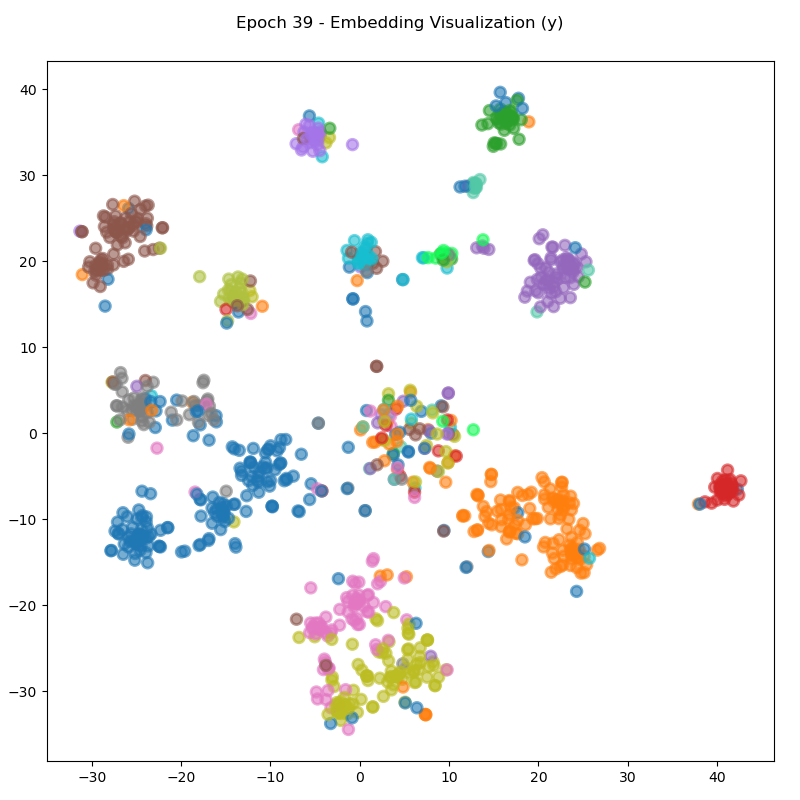
\includegraphics[width=0.23\columnwidth]{resources/visualization/ctdne_y.png} 
}
\subfigure[$CTDNE$ + $L_{\mathcal{T}}$]{
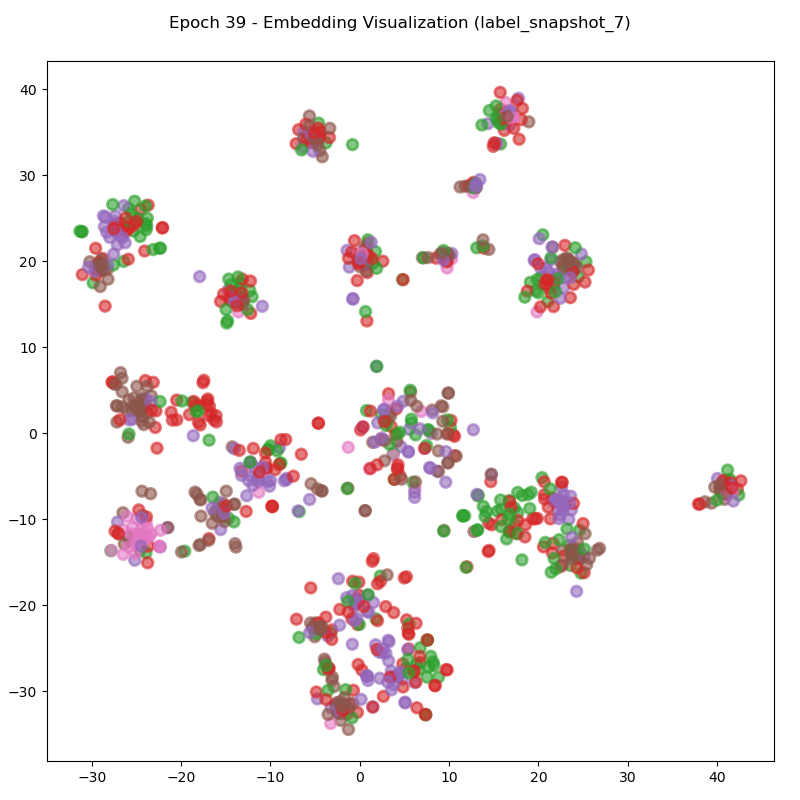
\includegraphics[width=0.23\columnwidth]{resources/visualization/ctdne_t.png}
}
\caption{Visualization of trained embedding against ground truth labels ($L_y$,  left) and timestamp labels ($L_{\mathcal{T}}$, right) for DBLP-HCN dataset.
(Note: The embeddings are calculated on the training dataset. Each of the plots contains a blob of nodes that have no edges in the training set due to the validation split. None of the methods is equipped to handle disconnected nodes.)
}
\label{fig:embeddings}
\end{figure*}    

We further compare $MGTCOM$ and the baseline models on the DBLP-HCN network.
We apply the T-SNE dimensionality reduction technique to visualize the trained node embeddings in 2D space colored by the ground truth label and the node timestamp (See \cref{fig:embeddings}).

Since in the DBLP-HCN dataset the timestamps are weakly correlated with its topology, we can see that topology-focused embedding (and community detection) methods such as ComE and Node2Vec do not capture temporal relations of nodes. On contrary, we observe distinct patterns emerge when looking at $MGTCOM$ generated embeddings for both of the labels.
%
Similar to that of $ComE$ the community structures are visible in the node embeddings though they are not as distinct.


%=====================================================================================
\section{Inference results}
Because the $MGTCOM$ model operates on sampled neighborhood subgraphs, in contrast to other methods it can operate in an inductive setting.
Meaning that it is not necessary to retrain the model to infer representation vectors for previously unseen nodes.

We evaluate the performance of $MGTCOM$ and its task-specific variants in inductive settings by controlling the ratio of nodes in the training set to the validation set.
The test set remains constant throughout the experiment to accurately assess performance on inferred nodes.
The relevant quality measures are computed exclusively on the test set and can be found in \cref{tab:results_inference}.

In \cref{fig:inference} we see the same measures plotted with the training ratio on the x-axis.
From \cref{fig:inference} (a) we observe that varying training set size does not affect link-prediction tasks as much as node classification tasks (b, c, d).
Throughout the measures, we can see that using only 75\% of the data does not substantially affect the results.
Interestingly, we observe that the variance on the temporal prediction task increases when more data is provided.

\begin{figure*}[t!]
\centering
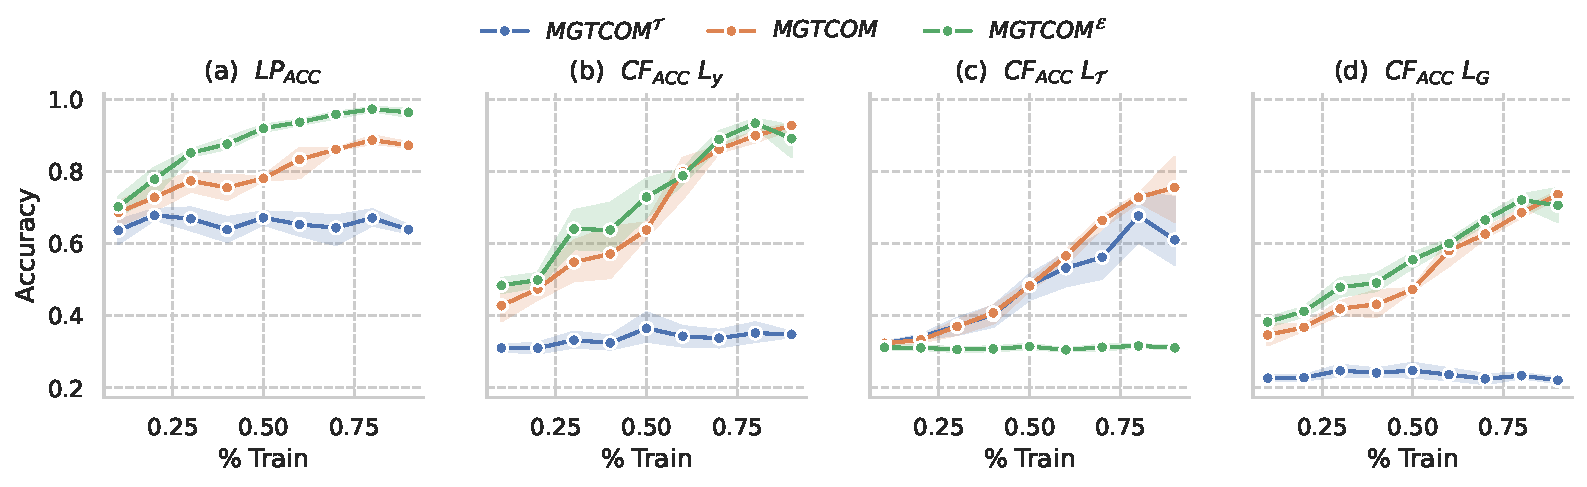
\includegraphics[width=\textwidth]{resources/figs/inference.pdf}
\caption{
    Visual comparison of different model variants in the inference-based setting. 
    Graph nodes are split into three disjointed sets (train, validation, and test).
    The metrics are measured while the training to validation ratio is varied. 
    The test set is set to 10\% of the nodes and is kept constant.
    The average metrics per data value are plotted along with their standard deviation.
}
\label{fig:inference}
\end{figure*}    
\begin{table*}[t!]
\centering
\caption{
    Comparison of different model variants in the inference-based setting. 
    Graph nodes are split into three disjointed sets (train, validation, and test).
    The metrics are measured while the training to validation ratio is varied. 
    The test set is set to 10\% of the nodes and is kept constant.
}
\label{tab:results_inference}
% \resizebox{\textwidth}{!}{
    \begin{tabular}{ll|ccccccccc}
    \toprule
     \textbf{Model}                      & \textbf{\% Train} &            10\% &            20\% &            30\% &            40\% &            50\% &            60\% &            70\% &            80\% &            90\% \\ 
    \midrule
$MGTCOM$ 
                       & $LP_{ACC}$ &  0.686 &  0.728 &  0.774 &  0.755 &  0.780 &  0.833 &  0.861 &  0.887 &  0.872 \\
                       & $CF_{ACC}$ $L_y$ &  0.428 &  0.474 &  0.548 &  0.571 &  0.638 &  0.799 &  0.861 &  0.899 &  0.927 \\
                       & $CF_{ACC}$ $L_\mathcal{T}$ &  0.323 &  0.333 &  0.370 &  0.408 &  0.483 &  0.566 &  0.664 &  0.728 &  0.755 \\
                       & $CF_{ACC}$ $L_G$ &  0.347 &  0.368 &  0.419 &  0.432 &  0.473 &  0.580 &  0.626 &  0.685 &  0.736 \\ \midrule
$MGTCOM^{\mathcal{E}}$ 
                       & $LP_{ACC}$ &  0.702 &  0.778 &  0.851 &  0.876 &  0.919 &  0.936 &  0.958 &  0.972 &  0.963 \\
                       & $CF_{ACC}$ $L_y$ &  0.484 &  0.499 &  0.640 &  0.637 &  0.729 &  0.788 &  0.888 &  0.933 &  0.891 \\
                       & $CF_{ACC}$ $L_\mathcal{T}$ &  0.312 &  0.311 &  0.306 &  0.308 &  0.314 &  0.305 &  0.312 &  0.316 &  0.311 \\
                       & $CF_{ACC}$ $L_G$ &  0.382 &  0.412 &  0.479 &  0.491 &  0.555 &  0.600 &  0.665 &  0.721 &  0.706 \\ \midrule
$MGTCOM^{\mathcal{T}}$ 
                       & $LP_{ACC}$ &  0.636 &  0.678 &  0.669 &  0.639 &  0.671 &  0.653 &  0.644 &  0.671 &  0.638 \\
                       & $CF_{ACC}$ $L_y$ &  0.310 &  0.310 &  0.332 &  0.324 &  0.365 &  0.343 &  0.337 &  0.352 &  0.348 \\
                       & $CF_{ACC}$ $L_\mathcal{T}$ &  0.323 &  0.341 &  0.372 &  0.403 &  0.485 &  0.532 &  0.562 &  0.677 &  0.610 \\
                       & $CF_{ACC}$ $L_G$ &  0.227 &  0.228 &  0.248 &  0.242 &  0.248 &  0.237 &  0.225 &  0.234 &  0.221 \\
    \bottomrule
    \end{tabular}

% }
\end{table*}


%=====================================================================================
\section{Learnable parameter reduction}
An important goal of our work is to prove that inductive-based community detection is feasible.
We address the structural similarity bias found in many unsupervised inductive algorithms by introducing a custom loss and sampling methodology in \cref{sec:obj_fn}.
While our model still utilizes embeddings to address the incompleteness constraints, we show in \cref{sec:abl:aux_emb} that importance-based pruning is an effective optimization to keep the model scalable.

As result, our model takes advantage of the scalability of inductive representation learning methods.
In \cref{tab:params} we compare the parameter count of the $MGTCOM$ model to the node2vec model which directly learns node embeddings.
Overall $MGTCOM$ has fewer parameters since the model size is bound by meta-topology.
In highly heterogeneous graphs such as the ICEWS dataset, the number of parameters may become larger than expected.
Specifically, the number of parameters is proportional to $|\mathcal{A}| + |\mathcal{R}|$.
For exact analysis on the number of learnable parameters the model uses, we refer the reader to \cref{sec:exact_params}. 

\begin{table}[ht!]
\centering
\caption{
    Parameter count comparison between node2vec and the $MGTCOM$ model.
    \label{tab:params}
}
% \resizebox{\columnwidth}{!}{
\small
\begin{tabular}{l|ll}
    \hline
    Dataset & node2vec  & $MGTCOM$  \\ \hline
    DBLP    & 683,968   & 173,910   \\
    ICEWS   & 669,632   & 1,072,302 \\
    IMDB    & 867,840   & 170,846   \\
    SDS     & 5,979,712 & 231,282   \\
    Cora    & 173,312   & 136,390   \\ \hline
\end{tabular}
% }
\end{table}